\section{Resultados}

Utilizamos o software \textit{SageMath 9.7} para realizar as análises, definindo diferentes parâmetros e condições iniciais para os modelos apresentados.

\subsection{Equilíbrios}

\begin{center}
\begin{tabular}{| c | c | c |}
\hline
%& \multicolumn{3}{c|}{Notas}\\
%\cline{2 - 7} % linha horizontal entre as colunas
% 2 e 4
Modelo & Sistema & Equilíbrios \\
\hline
Lotka-Volterra & 
$\left\{
\begin{array}{l}
\dfrac{dx}{dt}=x(a-by)\\
\dfrac{dy}{dt}=y(cx-d)
\end{array}
\right.$ & 
\begin{tabular}{c} 
$\left[ x = 0, y = 0 \right]$ \\
$\left[ x = \frac{d}{c}, y = \frac{a}{b} \right]$
\end{tabular} \\
\hline
Holling-Tanner & 
$\left\{
\begin{array}{l}
\dfrac{dx}{dt}=rx\left(1-\dfrac{x}{K}\right)-\dfrac{mxy}{A+x}\\
\dfrac{dy}{dt}=sy\left(1-\dfrac{cy}{x}\right)
\end{array}
\right.$ & 
\begin{tabular}{c} 
$\left[ x = 0, y = 0 \right]$ \\
$\left[ x = K, y = 0 \right]$ \\
$\left[ x = -A, y = 0 \right]$ \\
$\left[ x = - \frac{ \alpha + \sqrt{\beta} }{2cr}, y = -\frac{\alpha + \sqrt{\beta}}{2c^2r} \right]$ \\
$\left[ x = - \frac{ \alpha - \sqrt{\beta} }{2cr}, y = -\frac{\alpha - \sqrt{\beta}}{2c^2r} \right]$ \\
$\alpha = (A-K)cr + Km$ \\
\scriptsize{$\beta = (A+K)^2c^2r^2 + K^2m^2 + 2(AK - K^2)cmr$}
\end{tabular} \\
\hline
Rosenzweig-MacArthur & 
$\left\{
\begin{array}{l}
\dfrac{dx}{dt}=rx\left(1-\dfrac{x}{K}\right)-\dfrac{mxy}{A+x}\\
\dfrac{dy}{dt}=\dfrac{cmxy}{A+x}-sy
\end{array}
\right.$ & 
\begin{tabular}{c} 
$\left[ x = 0, y = 0 \right]$ \\
$\left[ x = K, y = 0 \right]$ \\
$\left[ x = -A, y = 0 \right]$ \\
$\left[ x = - \frac{ As }{cm - s}, y = \frac{AKc^2mr - (A^2 + AK)crs}{Kc^2m^2 - 2Kcms + Ks^2} \right]$ 
\end{tabular} \\
\hline
\end{tabular}
\end{center}

\subsection{Simulações}

%%%%%%%%%%%%%%%%%%%%%%%%%%%%%%%%%%%%%%%%%%%%%%%%%%%%%%%%%%%
%%%%%%%%%%%%%%%%%%%%%%%%%%%%%%%%%%%%%%%%%%%%%%%%%%%%%%%%%%%
%%%%%%%%%%%%%%%%%%%% Modelo L-V %%%%%%%%%%%%%%%%%%%%%%%%%%%
%%%%%%%%%%%%%%%%%%%%%%%%%%%%%%%%%%%%%%%%%%%%%%%%%%%%%%%%%%%
%%%%%%%%%%%%%%%%%%%%%%%%%%%%%%%%%%%%%%%%%%%%%%%%%%%%%%%%%%%

\subsubsection{Modelo de Lotka-Volterra}

Define-se os parâmetros $a = 0.0126, b = 0.0000101, c = 0.00012, d = 0.1534$, calculados por Isaías de Jesus, em sua dissertação de mestrado \cite{ij_2018} (2018). Nesse caso, temos os equilíbrios $P_1 = \left(0,0 \right)$ e $P_2 = \left( \frac{3835}{3}, \frac{126000}{101} \right)$, onde a matriz Jacobiana de $P_1$ tem autovalores $-\frac{767}{5000}$ e $\frac{63}{5000}$. Logo, $P_1$ é um ponto de sela. Já a Jacobiana de $P_2$ possui autovalores complexos com parte real nula e, portanto, $P_2$ é um centro. A seguir, tem-se a simulação para diferentes condições iniciais e seus respectivos planos de fase.

\begin{figure}[H]
    \centering
    \begin{subfigure}{0.4\textwidth}
        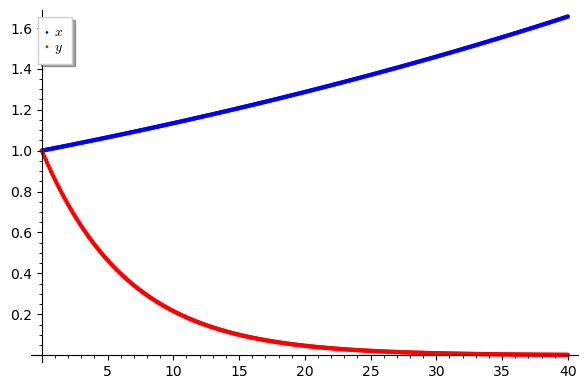
\includegraphics[scale=0.48]{figuras/LV_1.png}
        \label{fig:LV_1}
        \caption{$x_0 = y_0 = 1$}
    \end{subfigure}
    \begin{subfigure}{0.4\textwidth}
        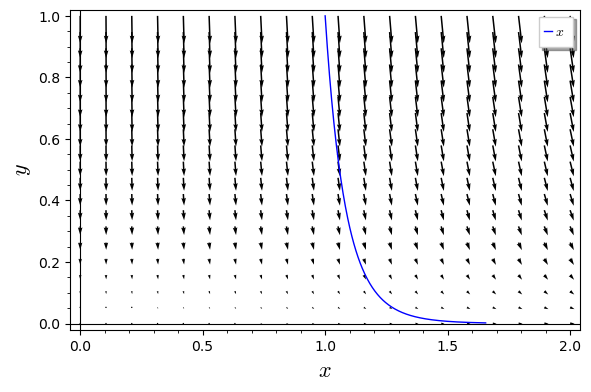
\includegraphics[scale=0.48]{figuras/LV_4.png}
        \label{fig:LV_4}
        \caption{Plano de fase}
    \end{subfigure}
\end{figure}

\begin{figure}[H]
    \centering
    \begin{subfigure}{0.4\textwidth}
        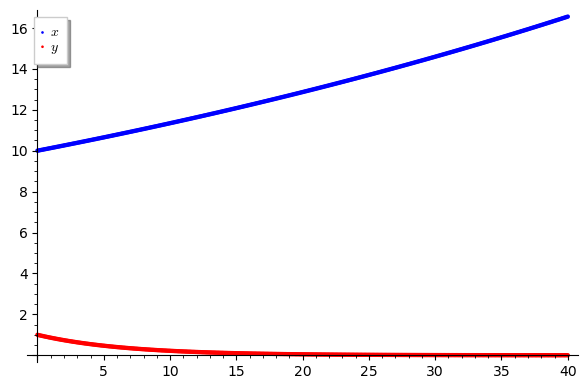
\includegraphics[scale=0.48]{figuras/LV_2.png}
        \label{fig:LV_2}
        \caption{$x_0 = 10$ e $y_0 = 1$}
    \end{subfigure}
    \begin{subfigure}{0.4\textwidth}
        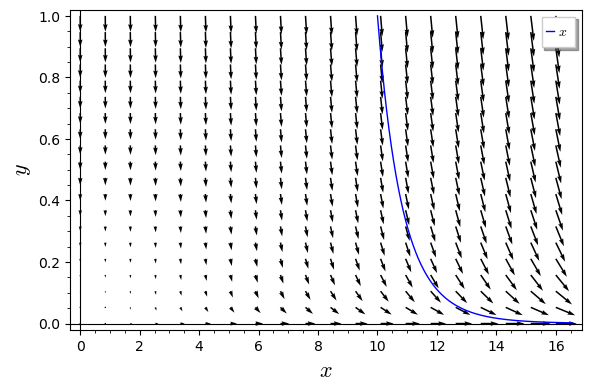
\includegraphics[scale=0.48]{figuras/LV_5.png}
        \label{fig:LV_5}
        \caption{Plano de fase}
    \end{subfigure}
\end{figure}

\begin{figure}[H]
    \centering
    \begin{subfigure}{0.4\textwidth}
        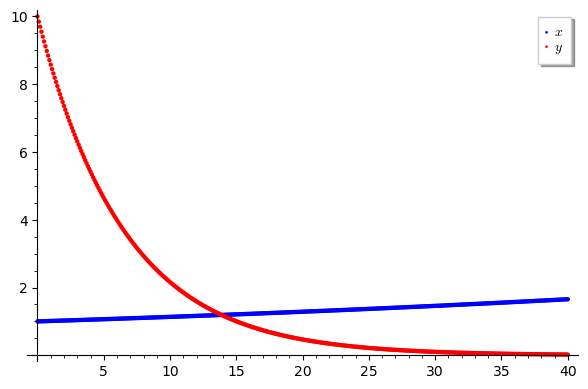
\includegraphics[scale=0.48]{figuras/LV_3.png}
        \label{fig:LV_3}
        \caption{$x_0 = 1$ e $y_0 = 10$}
    \end{subfigure}
    \begin{subfigure}{0.4\textwidth}
        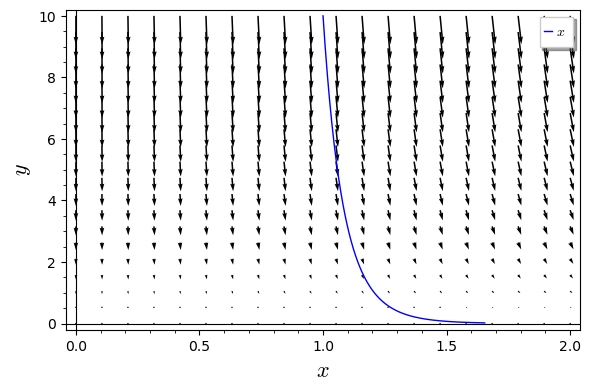
\includegraphics[scale=0.48]{figuras/LV_6.png}
        \label{fig:LV_6}
        \caption{Plano de fase}
    \end{subfigure}
\end{figure}

Quando variamos os parâmetros para $a = 0.0126, b = 0.01, c = 0.02, d = 0.0001$, vamos obter os seguintes gráficos.

\begin{figure}[H]
    \centering
    \begin{subfigure}{0.4\textwidth}
        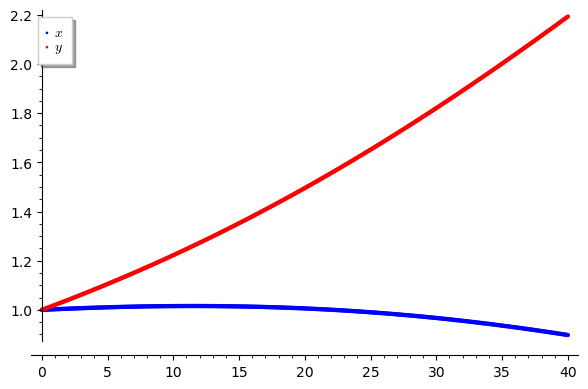
\includegraphics[scale=0.48]{figuras/LV_7.png}
        \label{fig:LV_7}
        \caption{$x_0 = y_0 = 1$}
    \end{subfigure}
    \begin{subfigure}{0.4\textwidth}
        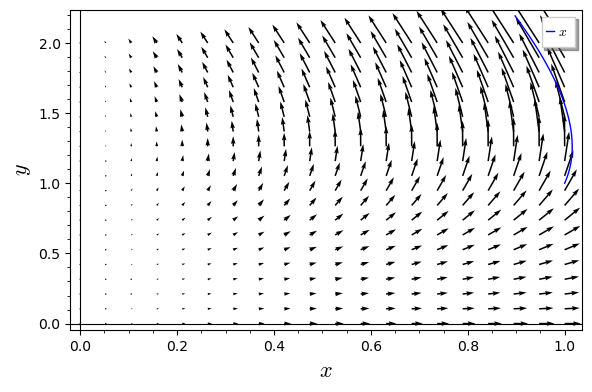
\includegraphics[scale=0.48]{figuras/LV_8.png}
        \label{fig:LV_8}
        \caption{Plano de fase}
    \end{subfigure}
\end{figure}

\begin{figure}[H]
    \centering
    \begin{subfigure}{0.4\textwidth}
        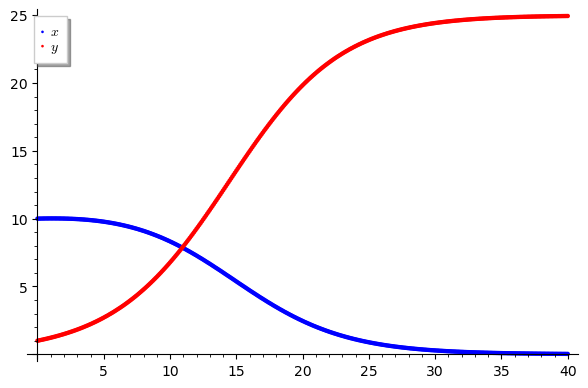
\includegraphics[scale=0.48]{figuras/LV_9.png}
        \label{fig:LV_9}
        \caption{$x_0 = 10$ e $y_0 = 1$}
    \end{subfigure}
    \begin{subfigure}{0.4\textwidth}
        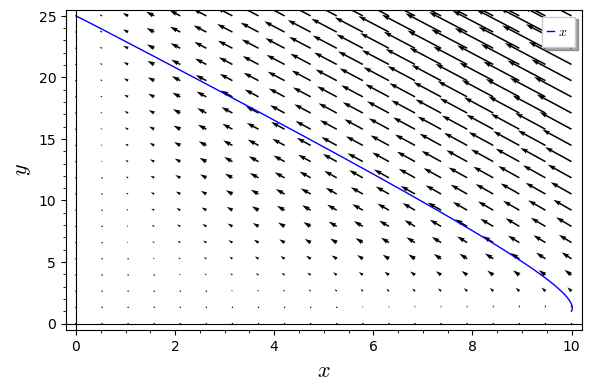
\includegraphics[scale=0.48]{figuras/LV_10.png}
        \label{fig:LV_10}
        \caption{Plano de fase}
    \end{subfigure}
\end{figure}

\begin{figure}[H]
    \centering
    \begin{subfigure}{0.4\textwidth}
        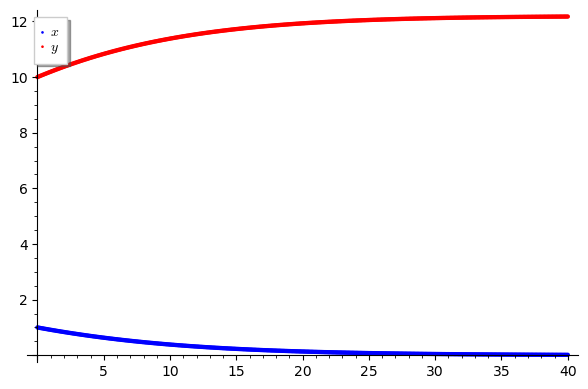
\includegraphics[scale=0.48]{figuras/LV_11.png}
        \label{fig:LV_11}
        \caption{$x_0 = 1$ e $y_0 = 10$}
    \end{subfigure}
    \begin{subfigure}{0.4\textwidth}
        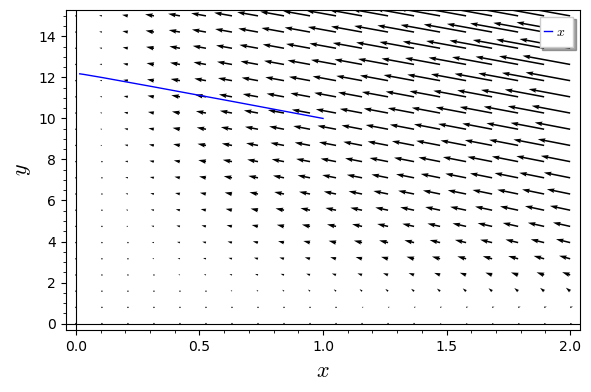
\includegraphics[scale=0.48]{figuras/LV_12.png}
        \label{fig:LV_12}
        \caption{Plano de fase}
    \end{subfigure}
\end{figure}

%%%%%%%%%%%%%%%%%%%%%%%%%%%%%%%%%%%%%%%%%%%%%%%%%%%%%%%%%%%
%%%%%%%%%%%%%%%%%%%%%%%%%%%%%%%%%%%%%%%%%%%%%%%%%%%%%%%%%%%
%%%%%%%%%%%%%%%%%%%% Modelo H-T %%%%%%%%%%%%%%%%%%%%%%%%%%%
%%%%%%%%%%%%%%%%%%%%%%%%%%%%%%%%%%%%%%%%%%%%%%%%%%%%%%%%%%%
%%%%%%%%%%%%%%%%%%%%%%%%%%%%%%%%%%%%%%%%%%%%%%%%%%%%%%%%%%%

\subsubsection{Modelo de Holling-Tanner}

Para esse modelo, os parâmetros foram calculados por M. S. Peixoto, L. C. Barros, e R. C. Bassanezi, no artigo produzido por eles \cite{mp_lb_rb_2005} (2005): $A = 10, K = 200, r = 2, m = 30.625, s = 0.3, c = 22.142857$. Nesse caso, temos os equilíbrios $P_1 = \left(0,0 \right), P_2 = \left( 200, 0 \right), P_3 = \left( -10, 0 \right), P_4 \approx \left( -25,806; -1,165 \right)$ e $P_5 \approx \left( 77,5; 3,5 \right)$, onde $P_2$ e $P_4$ são pontos de sela e $P_5$, uma espiral instável. A seguir, tem-se a simulação para diferentes condições iniciais e seus respectivos planos de fase.

\begin{figure}[H]
    \centering
    \begin{subfigure}{0.4\textwidth}
        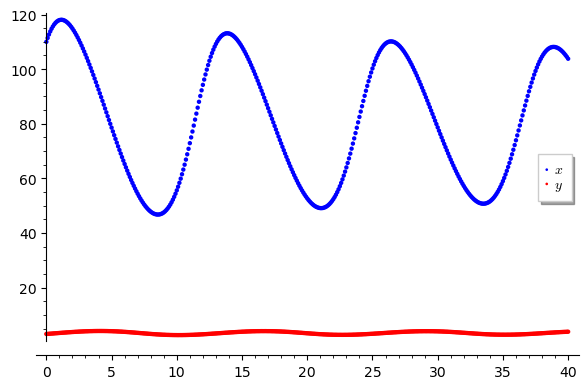
\includegraphics[scale=0.48]{figuras/HT_1.png}
        \label{fig:HT_1}
        \caption{$x_0 = 110$ e $y_0 = 3$}
    \end{subfigure}
    \begin{subfigure}{0.4\textwidth}
        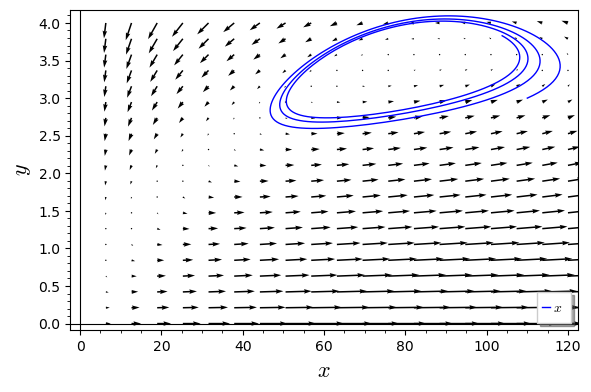
\includegraphics[scale=0.48]{figuras/HT_2.png}
        \label{fig:HT_2}
        \caption{Plano de fase}
    \end{subfigure}
\end{figure}

\begin{figure}[H]
    \centering
    \begin{subfigure}{0.4\textwidth}
        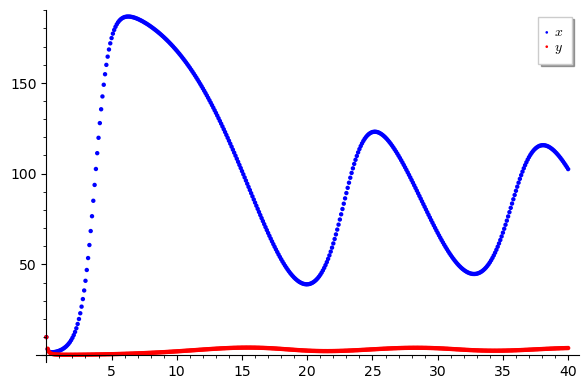
\includegraphics[scale=0.48]{figuras/HT_3.png}
        \label{fig:HT_3}
        \caption{$x_0 = y_0 = 10$}
    \end{subfigure}
    \begin{subfigure}{0.4\textwidth}
        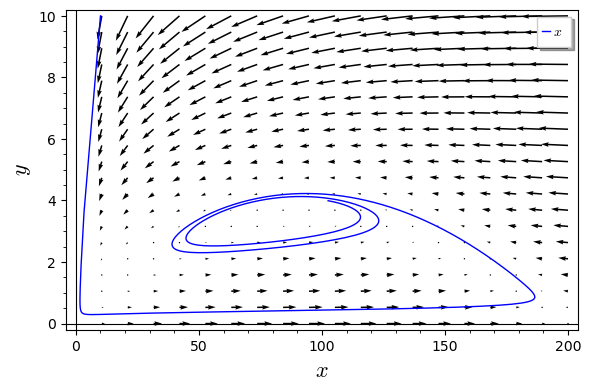
\includegraphics[scale=0.48]{figuras/HT_4.png}
        \label{fig:HT_4}
        \caption{Plano de fase}
    \end{subfigure}
\end{figure}

\begin{figure}[H]
    \centering
    \begin{subfigure}{0.4\textwidth}
        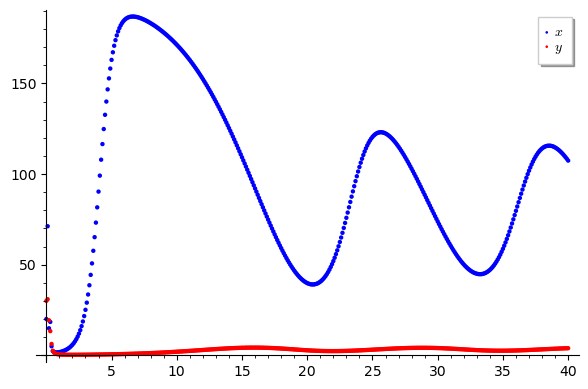
\includegraphics[scale=0.48]{figuras/HT_5.png}
        \label{fig:HT_5}
        \caption{$x_0 = 20$ e $y_0 = 30$}
    \end{subfigure}
    \begin{subfigure}{0.4\textwidth}
        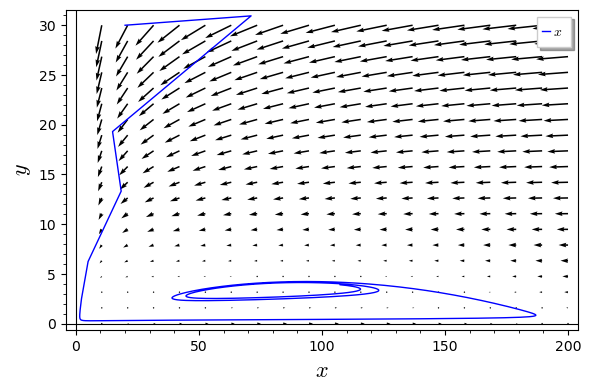
\includegraphics[scale=0.48]{figuras/HT_6.png}
        \label{fig:HT_6}
        \caption{Plano de fase}
    \end{subfigure}
\end{figure}

Quando aumentamos $s$ para $0.8$ e diminuímos $r$ para $1$, temos as seguintes figuras:

\begin{figure}[H]
    \centering
    \begin{subfigure}{0.4\textwidth}
        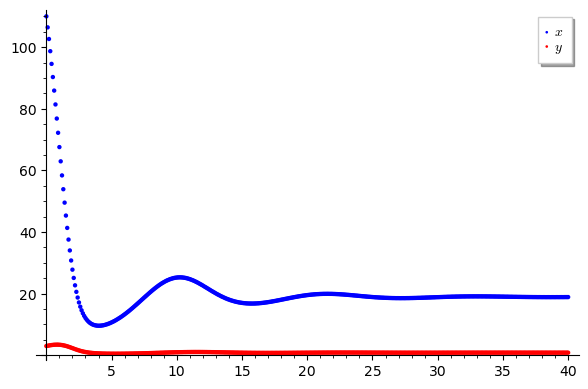
\includegraphics[scale=0.48]{figuras/HT_7.png}
        \label{fig:HT_7}
        \caption{$x_0 = 110$ e $y_0 = 3$}
    \end{subfigure}
    \begin{subfigure}{0.4\textwidth}
        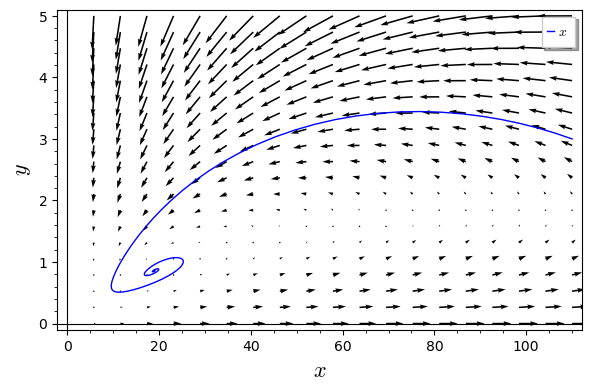
\includegraphics[scale=0.48]{figuras/HT_8.png}
        \label{fig:HT_8}
        \caption{Plano de fase}
    \end{subfigure}
\end{figure}

\begin{figure}[H]
    \centering
    \begin{subfigure}{0.4\textwidth}
        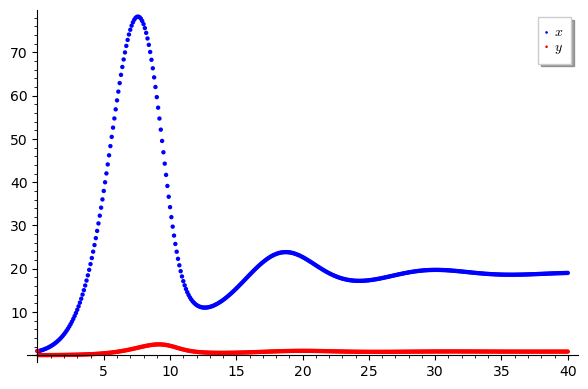
\includegraphics[scale=0.48]{figuras/HT_9.png}
        \label{fig:HT_9}
        \caption{$x_0 = y_0 = 1$}
    \end{subfigure}
    \begin{subfigure}{0.4\textwidth}
        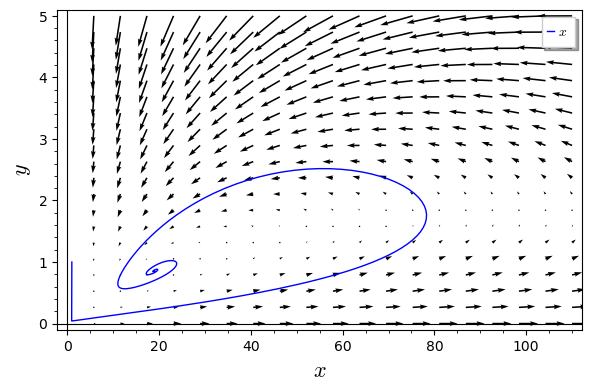
\includegraphics[scale=0.48]{figuras/HT_10.png}
        \label{fig:HT_10}
        \caption{Plano de fase}
    \end{subfigure}
\end{figure}

\begin{figure}[H]
    \centering
    \begin{subfigure}{0.4\textwidth}
        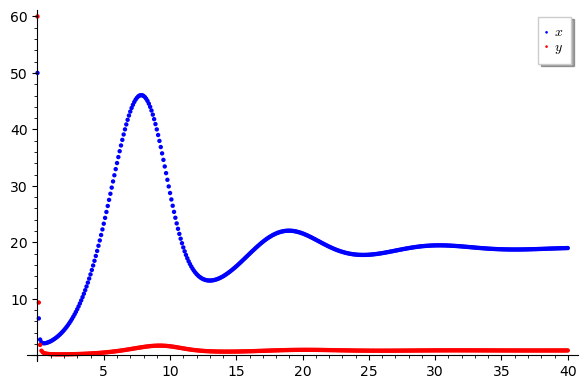
\includegraphics[scale=0.48]{figuras/HT_11.png}
        \label{fig:HT_11}
        \caption{$x_0 = 50$ e $y_0 = 60$}
    \end{subfigure}
    \begin{subfigure}{0.4\textwidth}
        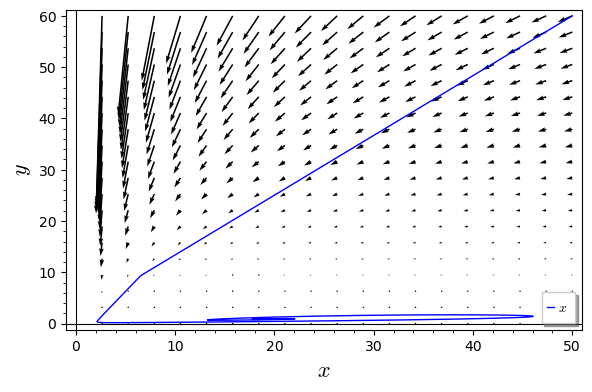
\includegraphics[scale=0.48]{figuras/HT_12.png}
        \label{fig:HT_12}
        \caption{Plano de fase}
    \end{subfigure}
\end{figure}

Por outro lado, aumentando também $m$ para $50$ e diminuindo $A$ para $5$, temos as seguintes figuras:

\begin{figure}[H]
    \centering
    \begin{subfigure}{0.4\textwidth}
        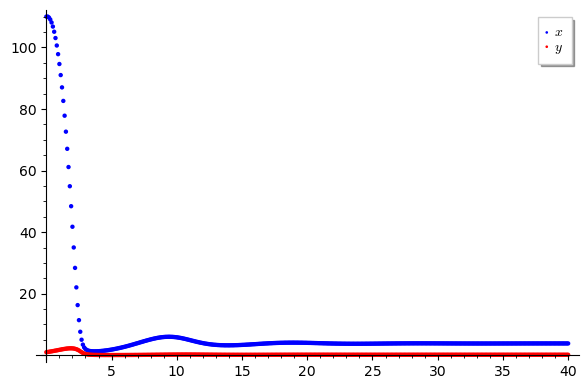
\includegraphics[scale=0.48]{figuras/HT_13.png}
        \label{fig:HT_13}
        \caption{$x_0 = 110$ e $y_0 = 1$}
    \end{subfigure}
    \begin{subfigure}{0.4\textwidth}
        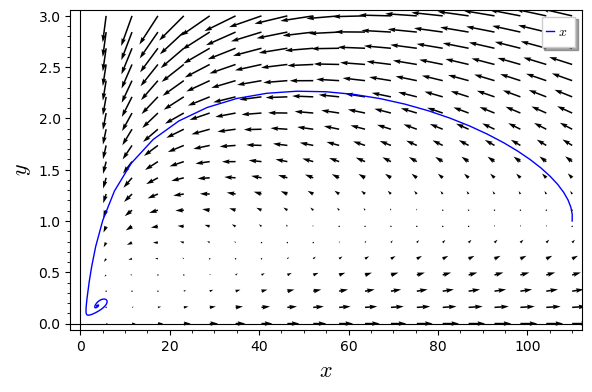
\includegraphics[scale=0.48]{figuras/HT_14.png}
        \label{fig:HT_14}
        \caption{Plano de fase}
    \end{subfigure}
\end{figure}

\begin{figure}[H]
    \centering
    \begin{subfigure}{0.4\textwidth}
        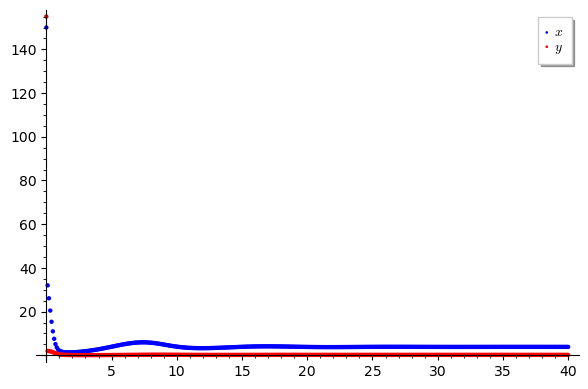
\includegraphics[scale=0.48]{figuras/HT_15.png}
        \label{fig:HT_15}
        \caption{$x_0 = 150$ e $y_0 = 155$}
    \end{subfigure}
    \begin{subfigure}{0.4\textwidth}
        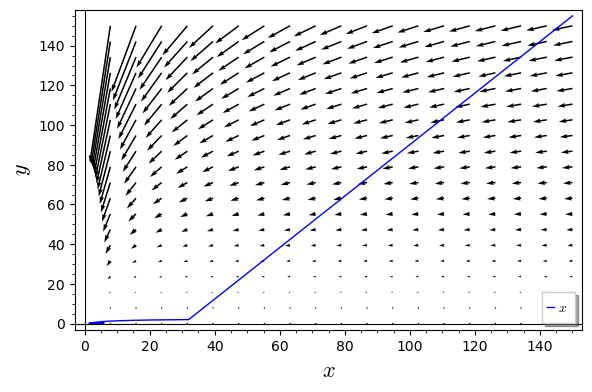
\includegraphics[scale=0.48]{figuras/HT_16.png}
        \label{fig:HT_16}
        \caption{Plano de fase}
    \end{subfigure}
\end{figure}

\begin{figure}[H]
    \centering
    \begin{subfigure}{0.4\textwidth}
        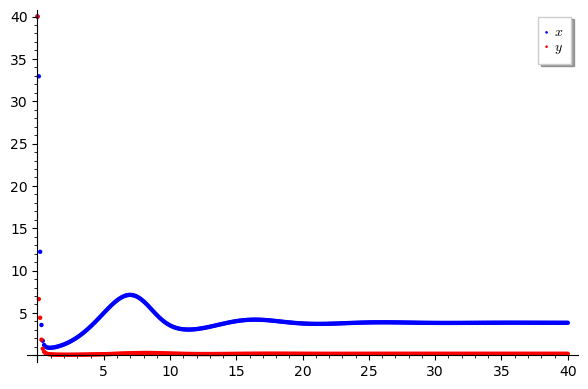
\includegraphics[scale=0.48]{figuras/HT_17.png}
        \label{fig:HT_17}
        \caption{$x_0 = y_0 = 40$}
    \end{subfigure}
    \begin{subfigure}{0.4\textwidth}
        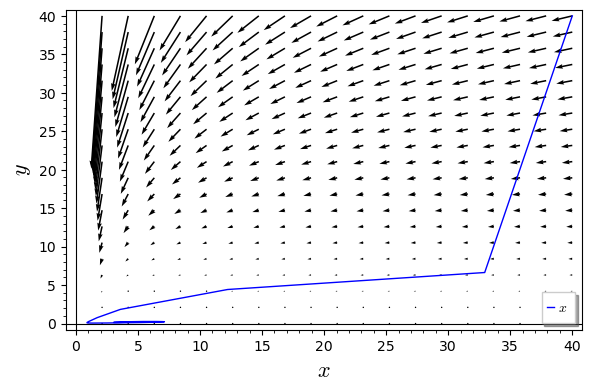
\includegraphics[scale=0.48]{figuras/HT_18.png}
        \label{fig:HT_18}
        \caption{Plano de fase}
    \end{subfigure}
\end{figure}

%%%%%%%%%%%%%%%%%%%%%%%%%%%%%%%%%%%%%%%%%%%%%%%%%%%%%%%%%%%
%%%%%%%%%%%%%%%%%%%%%%%%%%%%%%%%%%%%%%%%%%%%%%%%%%%%%%%%%%%
%%%%%%%%%%%%%%%%%%%% Modelo R-M %%%%%%%%%%%%%%%%%%%%%%%%%%%
%%%%%%%%%%%%%%%%%%%%%%%%%%%%%%%%%%%%%%%%%%%%%%%%%%%%%%%%%%%
%%%%%%%%%%%%%%%%%%%%%%%%%%%%%%%%%%%%%%%%%%%%%%%%%%%%%%%%%%%

\subsubsection{Modelo de Rosenzweig-MacArthur}

Nesse modelo, os parâmetros usados para o caso vespa-broca foram $A=5$, $K=100$, $r=1$, $m=15$, $s=0.45$ e $c=0.8$, testados nas populações iniciais $(x,y)=\{(1,1),(1,10),(10,1)\}$.

\begin{figure}[H]
    \centering
    \begin{subfigure}{0.4\textwidth}
        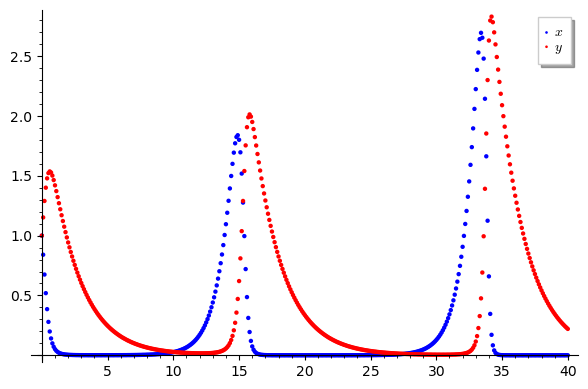
\includegraphics[scale=0.48]{figuras/RM-cana (1,1) plot.png}
        \label{fig:RM-cana_1}
        \caption{$x_0 = y_0 = 1$}
    \end{subfigure}
    \begin{subfigure}{0.4\textwidth}
        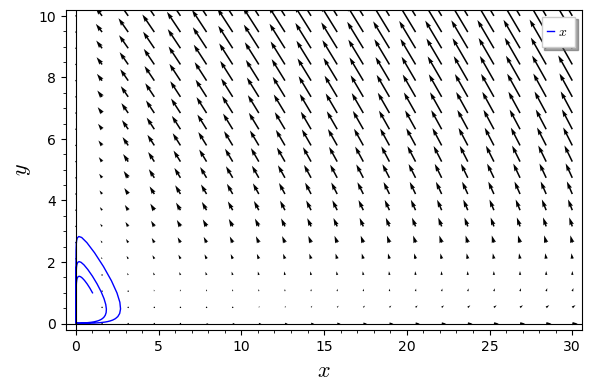
\includegraphics[scale=0.48]{figuras/RM-cana (1,1) plano.png}
        \label{fig:RM-cana_2}
        \caption{Plano de fase}
    \end{subfigure}
\end{figure}

\begin{figure}[H]
    \centering
    \begin{subfigure}{0.4\textwidth}
        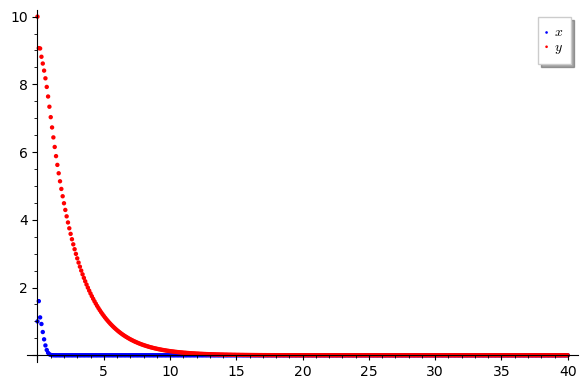
\includegraphics[scale=0.48]{figuras/RM-cana (1,10) plot.png}
        \label{fig:RM-cana_3}
        \caption{$x_0 = 1$ e $y_0 = 10$}
    \end{subfigure}
    \begin{subfigure}{0.4\textwidth}
        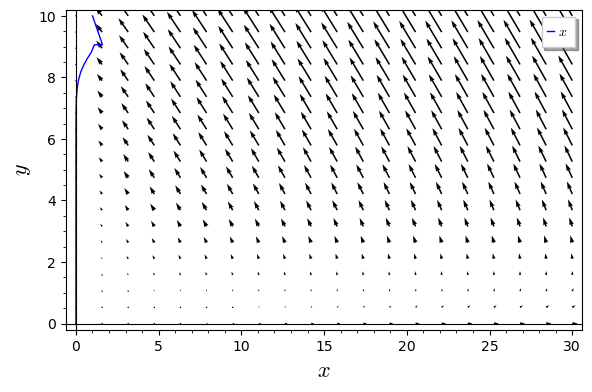
\includegraphics[scale=0.48]{figuras/RM-cana (1,10) plano.png}
        \label{fig:RM-cana_4}
        \caption{Plano de fase}
    \end{subfigure}
\end{figure}

\begin{figure}[H]
    \centering
    \begin{subfigure}{0.4\textwidth}
        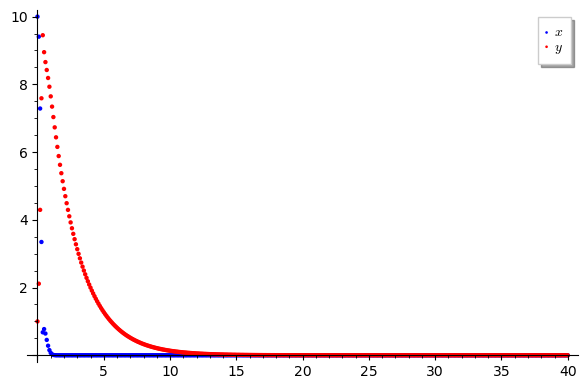
\includegraphics[scale=0.48]{figuras/RM-cana (10,1) plot.png}
        \label{fig:RM-cana_5}
        \caption{$x_0 = 10$ e $y_0 = 1$}
    \end{subfigure}
    \begin{subfigure}{0.4\textwidth}
        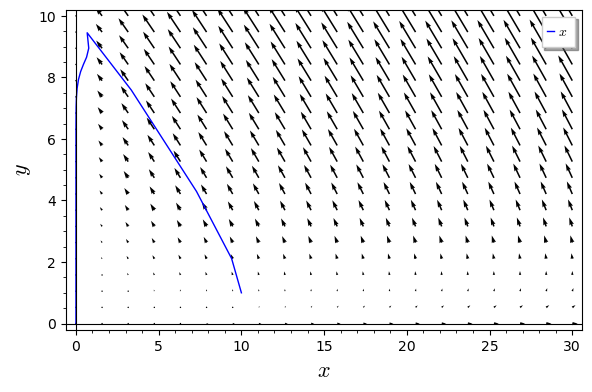
\includegraphics[scale=0.48]{figuras/RM-cana (10,1) plano.png}
        \label{fig:RM-cana_6}
        \caption{Plano de fase}
    \end{subfigure}
\end{figure}

Já no sistema joaninha-pulgão, os parâmetros utilizados foram $A=10$, $K=200$, $r=2$, $m=30.625$, $s=0.5$ e $c=1$, testados nas mesmas populações iniciais do caso anterior, $(x,y)=\{(1,1),(1,10),(10,1)\}$.

\begin{figure}[H]
    \centering
    \begin{subfigure}{0.4\textwidth}
        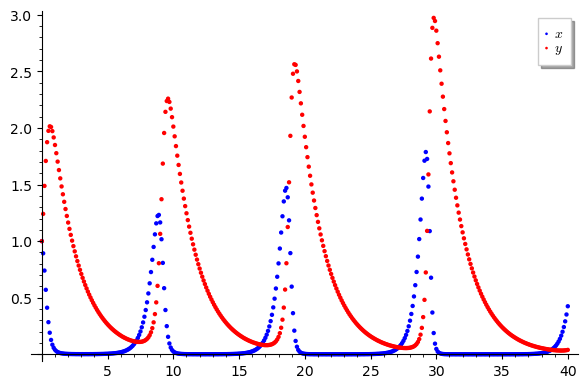
\includegraphics[scale=0.48]{figuras/RM-citros (1,1) plot.png}
        \label{fig:RM-citros_1}
        \caption{$x_0 = y_0 = 1$}
    \end{subfigure}
    \begin{subfigure}{0.4\textwidth}
        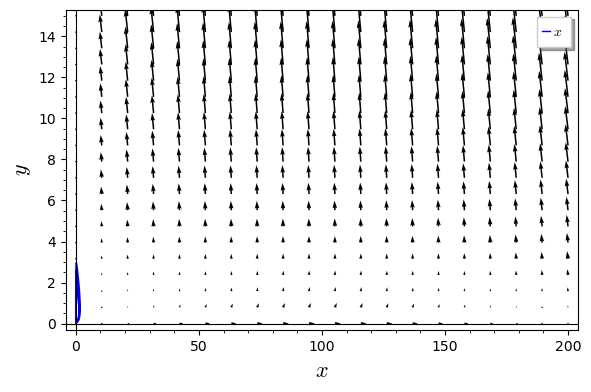
\includegraphics[scale=0.48]{figuras/RM-citros (1,1) plano.png}
        \label{fig:RM-citros_2}
        \caption{Plano de fase}
    \end{subfigure}
\end{figure}

\begin{figure}[H]
    \centering
    \begin{subfigure}{0.4\textwidth}
        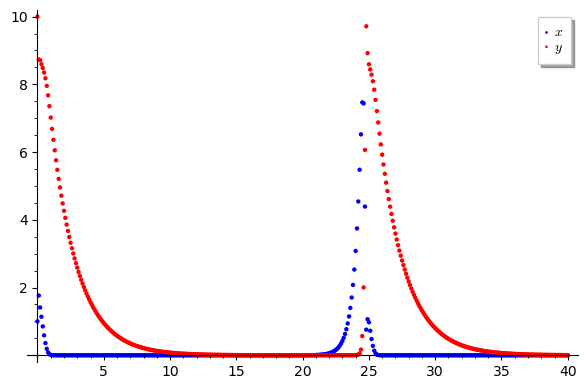
\includegraphics[scale=0.48]{figuras/RM-citros (1,10) plot.png}
        \label{fig:RM-citros_3}
        \caption{$x_0 = 1$ e $y_0 = 10$}
    \end{subfigure}
    \begin{subfigure}{0.4\textwidth}
        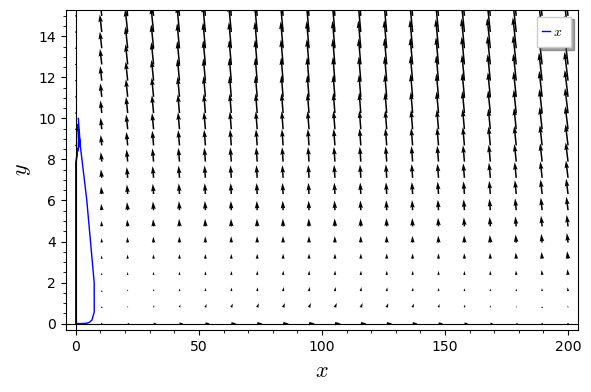
\includegraphics[scale=0.48]{figuras/RM-citros (1,10) plano.png}
        \label{fig:RM-citros_4}
        \caption{Plano de fase}
    \end{subfigure}
\end{figure}

\begin{figure}[H]
    \centering
    \begin{subfigure}{0.4\textwidth}
        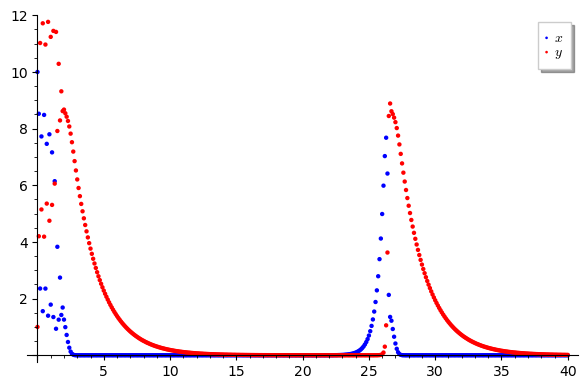
\includegraphics[scale=0.48]{figuras/RM-citros (10,1) plot.png}
        \label{fig:RM-citros_5}
        \caption{$x_0 = 10$ e $y_0 = 1$}
    \end{subfigure}
    \begin{subfigure}{0.4\textwidth}
        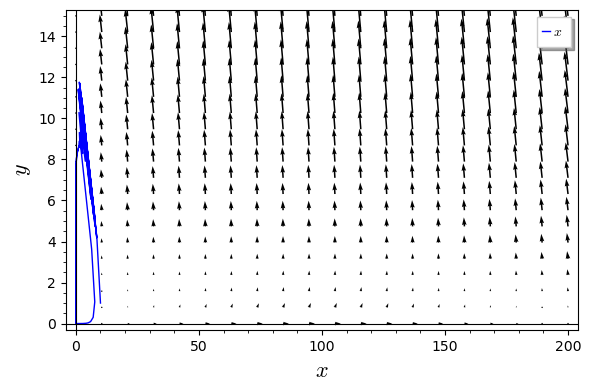
\includegraphics[scale=0.48]{figuras/RM-citros (10,1) plano.png}
        \label{fig:RM-citros_6}
        \caption{Plano de fase}
    \end{subfigure}
\end{figure}

A maneira como foi feita a estimação desses parâmetros será discutida na próxima seção.
